% Provenance (never printed): cycle 2 "Questionner l'espace et le temps"
% (the globe, the continents and the oceans, reading a world map); see
% sources/book1/PROVENANCE.md. Book 1, grade 3, chapter 2.
\chapter{Bola Dunia: Benua dan Samudra}\label{ch:g3:continents-and-oceans}

Di kelas Lena ada sebuah \omterm{def:g3:continents-and-oceans:globe}{bola dunia} di atas penyangganya. Lena memejamkan
mata, memutar \omterm{def:g3:continents-and-oceans:globe}{bola dunia} itu dengan satu jari, lalu menghentikannya dengan
ujung jarinya. Ia membuka mata: jarinya ada di warna biru, di tengah sebuah
\omterm{def:g2:water-on-earth:ocean}{samudra}. Ia mencoba lagi: biru lagi. Pada percobaan ketiga, jarinya
mendarat di warna hijau kekuningan, di suatu tempat di tengah Afrika.

Lena terus bermain, sambil menghitung. Jarinya jauh lebih sering berhenti di
\omterm{def:g2:water-on-earth:ocean}{laut} daripada di daratan. Mengapa? Dan apakah semua bentuk daratan dan
lautan yang berputar di bawah jarinya itu?

\begin{omfigure}
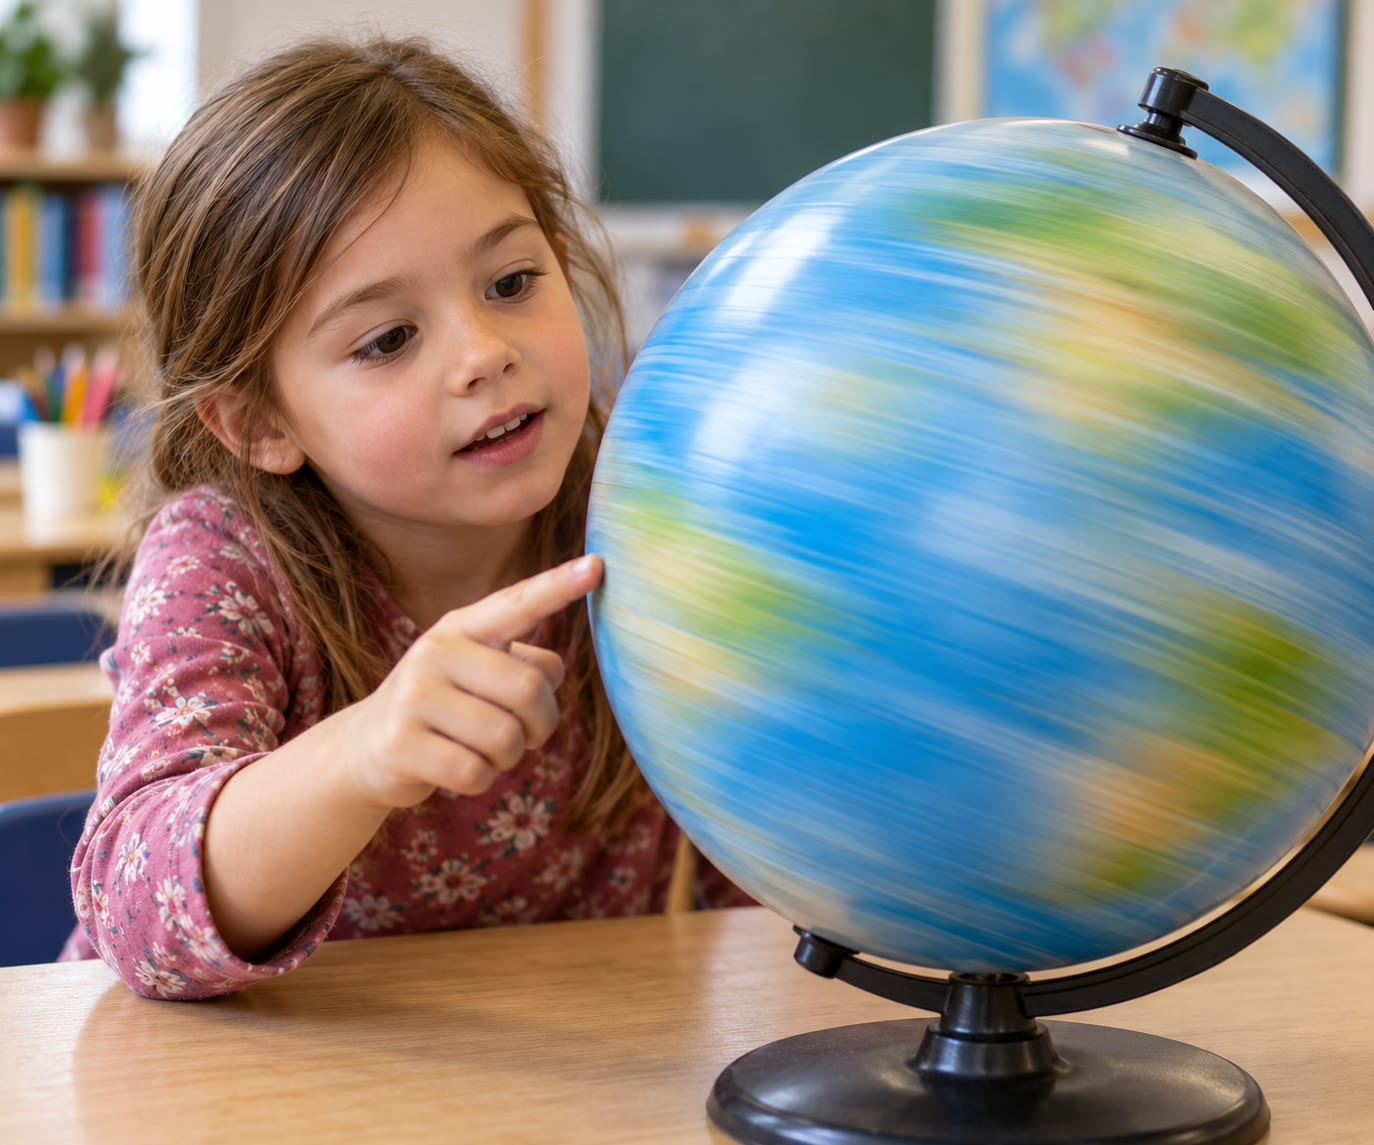
\includegraphics[width=0.6\linewidth]{images/book1/ai/g3-spinning-globe.jpg}

{\small \omterm{def:g3:continents-and-oceans:globe}{Bola dunia} yang berputar di atas penyangganya: daratan dan lautan
lewat di bawah jari.}
\end{omfigure}

\begin{recall}
Sebagian besar Bumi ditutupi \omterm{def:g2:water-on-earth:salt-fresh}{air asin}: sekitar 71 persegi dari 100 pada kisi
di \cref{ch:g2:water-on-earth}. \omterm{def:g2:water-on-earth:ocean}{Samudra} adalah hamparan \omterm{def:g2:water-on-earth:salt-fresh}{air asin} yang sangat
luas di antara daratan-daratan; \omterm{def:g2:water-on-earth:ocean}{laut} adalah hamparan yang lebih kecil, di
tepi \omterm{def:g2:water-on-earth:ocean}{samudra}. \omterm{def:g2:drawing-to-map:map}{Peta} adalah gambar sebuah tempat yang dilihat dari atas,
dibuat lebih kecil (\cref{ch:g2:drawing-to-map}). Buku fisika menceritakan
bagaimana Bumi berputar pada porosnya sekali sehari, yang memberi kita siang
dan malam.
\end{recall}

\section{Bola dunia, model kecil Bumi yang bulat}

Bumi itu bulat, seperti bola yang sangat besar. Kita tidak bisa melihat
bentuknya dari permukaan tanah, karena Bumi terlalu besar: di mana pun kita
berdiri, tanah tampak datar. Tetapi para astronaut yang pergi jauh dari
Bumi melihatnya secara utuh, sebuah bola biru yang bulat di langit yang
hitam (foto di awal \cref{ch:g2:water-on-earth}).

Untuk melihat seluruh Bumi di dalam kelas, kita membuatnya kecil.

\begin{definition}[Bola dunia]\label{def:g3:continents-and-oceans:globe}
Yang disebut \emph{bola dunia}\index{bola dunia} adalah model Bumi: sebuah
bola yang padanya digambar daratan dan \omterm{def:g2:water-on-earth:ocean}{samudra} dengan bentuk yang sama
seperti pada Bumi yang sebenarnya, hanya jauh lebih kecil.
\end{definition}

\omterm{def:g3:continents-and-oceans:globe}{Bola dunia} adalah gambaran Bumi yang paling baik, karena bentuknya benar:
bulat. Tetapi seperti Bumi yang sebenarnya, kita hanya bisa melihat
separuhnya pada satu waktu. Untuk melihat separuh yang lain, kita
memutarnya.

\begin{omfigure}
\begin{tikzpicture}
\begin{axis}[name=atl, hide axis, axis equal image, scale only axis,
    width=6.2cm, xmin=-1.05, xmax=1.05, ymin=-1.05, ymax=1.05, clip=false]
  \fill[omSea] (axis cs:0,0) circle[radius=1];
  \addplot[fill=omHypsLandA!85!black, draw=black!45, line width=0.2pt]
    table {figdata/out/grade-3-globe-atlantic-land.dat};
  \addplot[black!60, dashed, line width=0.5pt]
    table {figdata/out/grade-3-globe-atlantic-equator.dat};
  \addplot[only marks, mark=*, mark size=1.4pt, black]
    table[x=x, y=y] {figdata/out/grade-3-globe-atlantic-poles.dat};
  \node[font=\scriptsize, anchor=center, align=center, fill=white, fill opacity=0.7, text opacity=1, inner sep=1pt, rounded corners=1pt] at (axis cs:-0.683,0.636) {Amerika\\Utara};
  \node[font=\scriptsize, anchor=center, align=center, fill=white, fill opacity=0.7, text opacity=1, inner sep=1pt, rounded corners=1pt] at (axis cs:-0.561,-0.408) {Amerika\\Selatan};
  \node[font=\scriptsize, anchor=center, align=center, fill=white, fill opacity=0.7, text opacity=1, inner sep=1pt, rounded corners=1pt] at (axis cs:0.396,0.639) {Eropa};
  \node[font=\scriptsize, anchor=center, align=center, fill=white, fill opacity=0.7, text opacity=1, inner sep=1pt, rounded corners=1pt] at (axis cs:0.704,-0.098) {Afrika};
  \node[font=\scriptsize, anchor=center, align=center, fill=white, fill opacity=0.7, text opacity=1, inner sep=1pt, rounded corners=1pt] at (axis cs:-0.209,0.128) {Samudra\\Atlantik};
  \draw[black!70, line width=0.8pt] (axis cs:0,0) circle[radius=1];
  \node[font=\scriptsize, anchor=south] at (axis cs:0,0.97) {Kutub Utara};
\end{axis}
\begin{axis}[at={(atl.east)}, anchor=west, xshift=0.6cm, hide axis,
    axis equal image, scale only axis,
    width=6.2cm, xmin=-1.05, xmax=1.05, ymin=-1.05, ymax=1.05, clip=false]
  \fill[omSea] (axis cs:0,0) circle[radius=1];
  \addplot[fill=omHypsLandA!85!black, draw=black!45, line width=0.2pt]
    table {figdata/out/grade-3-globe-pacific-land.dat};
  \addplot[black!60, dashed, line width=0.5pt]
    table {figdata/out/grade-3-globe-pacific-equator.dat};
  \node[font=\scriptsize, anchor=center, align=center, fill=white, fill opacity=0.7, text opacity=1, inner sep=1pt, rounded corners=1pt] at (axis cs:-0.754,-0.391) {Australia};
  \node[font=\scriptsize, anchor=center, align=center, fill=white, fill opacity=0.7, text opacity=1, inner sep=1pt, rounded corners=1pt] at (axis cs:0.258,0.087) {Samudra\\Pasifik};
  \draw[black!70, line width=0.8pt] (axis cs:0,0) circle[radius=1];
\end{axis}
\end{tikzpicture}

{\small \omterm{def:g3:continents-and-oceans:globe}{Bola dunia} dilihat dari dua sisi. Kiri: sisi \omterm{def:g2:water-on-earth:ocean}{Samudra} Atlantik,
dengan benua Amerika, Eropa, dan Afrika. Kanan: sisi yang lain, \omterm{def:g2:water-on-earth:ocean}{Samudra}
Pasifik, dengan Australia di tepinya. Garis putus-putus adalah
\omterm{def:g3:continents-and-oceans:equator}{khatulistiwa}. Garis pantai: Natural Earth (domain publik).}
\label{fig:g3:continents-and-oceans:globes}
% ledger: data:ne-land
\end{omfigure}

\begin{remark}[Dua belahan yang sangat berbeda]\label{rem:g3:continents-and-oceans:halves}
Lihatlah kedua gambar itu. Di sebelah kiri, daratan menutupi sekitar 4
bagian dari 10 bagian gambar. Di sebelah kanan, hanya sekitar 1 bagian
dari 10: sisi Pasifik Bumi hampir seluruhnya air. Jika jari Lena berhenti
di sisi \omterm{def:g3:continents-and-oceans:globe}{bola dunia} itu, jarinya hampir selalu mendarat di \omterm{def:g2:water-on-earth:ocean}{laut}.
\end{remark}

\section{Khatulistiwa, kutub, dan kedua belahan bumi}

\omterm{def:g3:continents-and-oceans:globe}{Bola dunia} berputar pada sebatang poros yang menembusnya, dari atas sampai
ke bawah. Bumi yang sebenarnya tidak mempunyai batang poros, tetapi Bumi
juga berputar mengelilingi sebuah garis yang melewati bagian tengahnya.
Kedua tempat garis itu keluar dari Bumi mempunyai nama.

\begin{definition}[Kutub]\label{def:g3:continents-and-oceans:poles}
\emph{Kutub Utara}\index{Kutub Utara} dan \emph{Kutub
Selatan}\index{Kutub Selatan} adalah dua titik di bagian paling atas dan
paling bawah Bumi, tempat keluarnya garis yang menjadi poros perputaran
Bumi. Masing-masing disebut sebuah \emph{kutub}\index{kutub}. Pada \omterm{def:g3:continents-and-oceans:globe}{bola
dunia}, Kutub Utara ada di atas.
\end{definition}

\begin{definition}[Khatulistiwa dan belahan bumi]\label{def:g3:continents-and-oceans:equator}
Yang disebut \emph{khatulistiwa}\index{khatulistiwa} adalah garis khayal
yang digambar melingkari Bumi, tepat di tengah-tengah antara \omterm{def:g3:continents-and-oceans:poles}{Kutub Utara}
dan \omterm{def:g3:continents-and-oceans:poles}{Kutub Selatan}. Garis itu membagi Bumi menjadi dua bagian, yang
masing-masing disebut \emph{belahan bumi}\index{belahan bumi}:
\emph{belahan bumi utara}\index{belahan bumi utara}, di sisi \omterm{def:g3:continents-and-oceans:poles}{Kutub Utara},
dan \emph{belahan bumi selatan}\index{belahan bumi selatan}, di sisi \omterm{def:g3:continents-and-oceans:poles}{Kutub
Selatan}.
\end{definition}

\omterm{def:g3:continents-and-oceans:equator}{Khatulistiwa} tidak dicat di tanah: tak seorang pun bisa melihatnya di
pantai atau di hutan. Garis itu digambar pada \omterm{def:g3:continents-and-oceans:globe}{bola dunia} dan \omterm{def:g2:drawing-to-map:map}{peta} untuk
membantu kita menemukan jalan.

\begin{omfigure}
\begin{tikzpicture}[font=\small]
  % globe outline
  \fill[omSea!70] (0,0) circle (2.2);
  % northern hemisphere tinted
  \begin{scope}
    \clip (0,0) circle (2.2);
    \fill[yellow!25, opacity=0.8] (-2.3,0) -- (-2.3,2.3) -- (2.3,2.3) -- (2.3,0)
      arc[start angle=0, end angle=-180, x radius=2.3, y radius=0.45] -- cycle;
  \end{scope}
  \draw[black!70, line width=0.8pt] (0,0) circle (2.2);
  % equator: front half solid, back half dashed
  \draw[red!70!black, line width=1.2pt] (-2.2,0) arc[start angle=180, end angle=360, x radius=2.2, y radius=0.4];
  \draw[red!70!black, line width=0.8pt, dashed] (2.2,0) arc[start angle=0, end angle=180, x radius=2.2, y radius=0.4];
  % axis and poles
  \draw[black!60, line width=0.6pt] (0,2.2) -- (0,2.75);
  \draw[black!60, line width=0.6pt] (0,-2.2) -- (0,-2.75);
  \draw[black!60, line width=0.6pt, dotted] (0,2.2) -- (0,-2.2);
  \fill (0,2.2) circle (2.2pt);
  \fill (0,-2.2) circle (2.2pt);
  \node[anchor=west] at (0.15,2.6) {Kutub Utara};
  \node[anchor=west] at (0.15,-2.6) {Kutub Selatan};
  % labels
  \node[anchor=west] at (2.6,0) {khatulistiwa};
  \draw[black!60] (2.55,0) -- (2.05,-0.15);
  \node[anchor=west, align=left] at (2.6,1.4) {belahan\\bumi utara};
  \draw[black!60] (2.55,1.4) -- (1.5,1.2);
  \node[anchor=west, align=left] at (2.6,-1.4) {belahan\\bumi selatan};
  \draw[black!60] (2.55,-1.4) -- (1.5,-1.2);
\end{tikzpicture}

{\small \omterm{def:g3:continents-and-oceans:equator}{Khatulistiwa} membagi Bumi menjadi dua \omterm{def:g3:continents-and-oceans:equator}{belahan bumi}. \omterm{def:g3:continents-and-oceans:equator}{Belahan bumi
utara} (diwarnai) ada di sisi \omterm{def:g3:continents-and-oceans:poles}{Kutub Utara}, \omterm{def:g3:continents-and-oceans:equator}{belahan bumi selatan} di sisi
\omterm{def:g3:continents-and-oceans:poles}{Kutub Selatan}.}
\label{fig:g3:continents-and-oceans:hemispheres}
\end{omfigure}

\begin{example}[Panas di dekat khatulistiwa, dingin di dekat kutub]\label{ex:g3:continents-and-oceans:hot-cold}
Daratan di dekat \omterm{def:g3:continents-and-oceans:equator}{khatulistiwa} panas sepanjang tahun: di sanalah hutan
hujan yang luas tumbuh. Daratan di dekat \omterm{def:g3:continents-and-oceans:poles}{kutub} dingin sepanjang tahun, dan
sebagian besar ditutupi es. Di tahun berikutnya kamu akan mempelajari
mengapa demikian; untuk sekarang, ingatlah: makin dekat ke \omterm{def:g3:continents-and-oceans:poles}{kutub}, makin
dingin.
\end{example}

\section{Tujuh benua dan lima samudra}

Pada \omterm{def:g3:continents-and-oceans:globe}{bola dunia}, daratan tidak tersebar dalam potongan-potongan kecil di
mana-mana. Sebagian besar daratan berkumpul dalam beberapa bongkahan yang
sangat besar.

\begin{definition}[Benua]\label{def:g3:continents-and-oceans:continent}
Yang disebut \emph{benua}\index{benua} adalah salah satu daratan yang sangat
luas di Bumi, bersama pulau-pulau yang dekat dengannya.
\end{definition}

Orang paling sering menghitung tujuh \omterm{def:g3:continents-and-oceans:continent}{benua}. Dari yang terbesar sampai yang
terkecil, \omterm{def:g3:continents-and-oceans:continent}{benua-benua} itu adalah: Asia, Afrika, Amerika Utara, Amerika
Selatan, Antarktika, Eropa, dan Australia.
% ledger: natgeo:seven-continents

\begin{center}\small
\begin{tabular}{rlll}
\hline
Ukuran & \omterm{def:g3:continents-and-oceans:continent}{Benua} & \omterm{def:g3:continents-and-oceans:equator}{Belahan bumi} & Sekilas tentang \omterm{def:g3:continents-and-oceans:continent}{benua} itu \\
\hline
1 & Asia & sebagian besar utara & yang terbesar \\
2 & Afrika & keduanya & \omterm{def:g3:continents-and-oceans:equator}{khatulistiwa} melintasi bagian tengahnya \\
3 & Amerika Utara & utara & membentang jauh ke utara \\
4 & Amerika Selatan & sebagian besar selatan & \omterm{def:g3:continents-and-oceans:equator}{khatulistiwa} melintasi bagian utaranya \\
5 & Antarktika & selatan & di sekitar \omterm{def:g3:continents-and-oceans:poles}{Kutub Selatan}, di bawah es \\
6 & Eropa & utara & menyatu dengan Asia di sisi timurnya \\
7 & Australia & selatan & yang terkecil \\
\hline
\end{tabular}
\end{center}

\begin{remark}[Di mana sebuah benua berakhir?]\label{rem:g3:continents-and-oceans:where}
Sebagian \omterm{def:g3:continents-and-oceans:continent}{benua} dikelilingi \omterm{def:g2:water-on-earth:ocean}{laut} di semua sisinya, seperti Australia atau
Antarktika. \omterm{def:g3:continents-and-oceans:continent}{Benua} yang lain saling bersentuhan: Eropa dan Asia adalah satu
daratan yang utuh, dan oranglah yang memilih di mana garis di antara
keduanya ditarik. Itulah sebabnya ada orang yang menghitung enam \omterm{def:g3:continents-and-oceans:continent}{benua},
atau bahkan kurang.
\end{remark}

Di antara \omterm{def:g3:continents-and-oceans:continent}{benua-benua} terletak \omterm{def:g2:water-on-earth:ocean}{samudra-samudra}. Jumlahnya ada lima. Yang
terbesar adalah \emph{\omterm{def:g2:water-on-earth:ocean}{Samudra} Pasifik}; lalu \emph{\omterm{def:g2:water-on-earth:ocean}{Samudra} Atlantik},
\emph{\omterm{def:g2:water-on-earth:ocean}{Samudra} Hindia}, \emph{\omterm{def:g2:water-on-earth:ocean}{Samudra} Selatan} di sekitar Antarktika, dan
yang terkecil, \emph{\omterm{def:g2:water-on-earth:ocean}{Samudra} Arktik} di sekitar \omterm{def:g3:continents-and-oceans:poles}{Kutub Utara}. Lama sekali
orang hanya menghitung empat; sekarang kebanyakan negara menghitung
\omterm{def:g2:water-on-earth:ocean}{Samudra} Selatan sebagai \omterm{def:g2:water-on-earth:ocean}{samudra} kelima.
% ledger: nos:five-oceans, nos:pacific-largest, oer:arctic-smallest

\begin{example}[Seberapa luas Samudra Pasifik?]\label{ex:g3:continents-and-oceans:pacific}
\omterm{def:g2:water-on-earth:ocean}{Samudra} Pasifik begitu luas sehingga semua \omterm{def:g3:continents-and-oceans:continent}{benua} jika disatukan bisa muat di
dalamnya. \omterm{def:g2:water-on-earth:ocean}{Samudra} ini menampung lebih dari separuh seluruh air \omterm{def:g2:water-on-earth:ocean}{samudra} di
Bumi. Itulah sebabnya \omterm{def:g3:continents-and-oceans:globe}{bola dunia} sebelah kanan di subbab pertama bab ini
tampak hampir seluruhnya biru.
% ledger: nos:pacific-largest
\end{example}

\begin{method}[Menamai samudra di antara dua benua]\label{met:g3:continents-and-oceans:between}
Untuk mengetahui \omterm{def:g2:water-on-earth:ocean}{samudra} mana yang terletak di antara dua \omterm{def:g3:continents-and-oceans:continent}{benua}, letakkan
satu jari pada masing-masing \omterm{def:g3:continents-and-oceans:continent}{benua} itu di \omterm{def:g3:continents-and-oceans:globe}{bola dunia}, lalu putarlah \omterm{def:g3:continents-and-oceans:globe}{bola
dunia} itu sehingga kamu bisa melihat keduanya. \omterm{def:g2:water-on-earth:ocean}{Samudra} yang dilintasi
matamu untuk berpindah dari satu jari ke jari yang lain adalah \omterm{def:g2:water-on-earth:ocean}{samudra} di
antara keduanya. Pada \omterm{def:g3:continents-and-oceans:globe}{bola dunia} sering ada dua jalan memutar: ambillah
yang lebih pendek.
\end{method}

\begin{example}[Afrika dan Australia]\label{ex:g3:continents-and-oceans:africa-australia}
Dari Afrika ke arah timur menuju Australia, kita melintasi \omterm{def:g2:water-on-earth:ocean}{Samudra} Hindia.
Dari Eropa ke arah barat menuju Amerika Utara, kita melintasi \omterm{def:g2:water-on-earth:ocean}{Samudra}
Atlantik. Dari Asia ke arah timur menuju Amerika Utara, kita melintasi
\omterm{def:g2:water-on-earth:ocean}{Samudra} Pasifik.
\end{example}

\section{Peta dunia adalah bola dunia yang dibuat datar}

\omterm{def:g3:continents-and-oceans:globe}{Bola dunia} itu bulat, jadi tidak mudah dibawa ke mana-mana, dan kita tidak
pernah bisa melihat seluruhnya sekaligus. \omterm{def:g2:drawing-to-map:map}{Peta} di atas selembar kertas
menunjukkan seluruh Bumi dalam sekali pandang.

\begin{definition}[Peta dunia]\label{def:g3:continents-and-oceans:world-map}
Yang disebut \emph{peta dunia}\index{peta dunia} adalah \omterm{def:g2:drawing-to-map:map}{peta} seluruh Bumi
yang digambar datar di atas selembar kertas atau di layar, dengan semua
\omterm{def:g3:continents-and-oceans:continent}{benua} dan semua \omterm{def:g2:water-on-earth:ocean}{samudra} dalam satu gambar.
\end{definition}

\begin{omfigure}
\begin{tikzpicture}
\begin{axis}[ommap, width=0.97\linewidth, xtick=\empty, ytick={0},
    yticklabels={khatulistiwa}, grid=none, clip=true]
  \addplot[fill=omHypsLandA!85!black, draw=black!45, line width=0.2pt]
    table {figdata/out/shared-geo-land.dat};
  \draw[black!60, dashed, line width=0.5pt] (axis cs:-180,0) -- (axis cs:180,0);
  \begin{scope}[every node/.style={font=\scriptsize, align=center}]
    \node at (axis cs:-102,47) {Amerika\\Utara};
    \node at (axis cs:-60,-12) {Amerika\\Selatan};
    \node at (axis cs:17,52) {Eropa};
    \node at (axis cs:20,6) {Afrika};
    \node at (axis cs:92,48) {Asia};
    \node at (axis cs:134,-24) {Australia};
    \node at (axis cs:40,-80) {Antarktika};
  \end{scope}
  \begin{scope}[every node/.style={font=\scriptsize\itshape, align=center, text=omSea!35!black}]
    \node at (axis cs:-145,8) {Samudra\\Pasifik};
    \node at (axis cs:165,12) {Samudra\\Pasifik};
    \node at (axis cs:-38,22) {Samudra\\Atlantik};
    \node at (axis cs:-15,-25) {Samudra\\Atlantik};
    \node at (axis cs:78,-22) {Samudra\\Hindia};
    \node at (axis cs:-115,-57) {Samudra Selatan};
    \node at (axis cs:-150,79) {Samudra Arktik};
  \end{scope}
\end{axis}
\end{tikzpicture}

{\small \omterm{def:g3:continents-and-oceans:world-map}{Peta dunia}. \omterm{def:g3:continents-and-oceans:globe}{Bola dunia} dipotong sepanjang garis yang melewati
tengah \omterm{def:g2:water-on-earth:ocean}{Samudra} Pasifik lalu direntangkan menjadi datar: \omterm{def:g2:water-on-earth:ocean}{Samudra} Pasifik
muncul dua kali, di tepi kiri dan di tepi kanan. Antarktika, sebuah \omterm{def:g3:continents-and-oceans:continent}{benua}
bundar di sekitar \omterm{def:g3:continents-and-oceans:poles}{Kutub Selatan}, terentang menjadi pita panjang di
sepanjang bagian bawah. Garis pantai: Natural Earth (domain publik).}
\label{fig:g3:continents-and-oceans:world-map}
% ledger: data:ne-land
\end{omfigure}

Tetapi ada kesulitan. Cobalah meratakan kulit jeruk di atas meja: kulit itu
tidak bisa terletak datar tanpa robek atau meregang. Hal yang sama terjadi
pada permukaan \omterm{def:g3:continents-and-oceans:globe}{bola dunia} ketika digambar datar. Setiap \omterm{def:g3:continents-and-oceans:world-map}{peta dunia} merobek
\omterm{def:g3:continents-and-oceans:globe}{bola dunia} di suatu tempat, atau meregangkan beberapa tempat dan
memampatkan tempat-tempat lain.

\begin{omfigure}
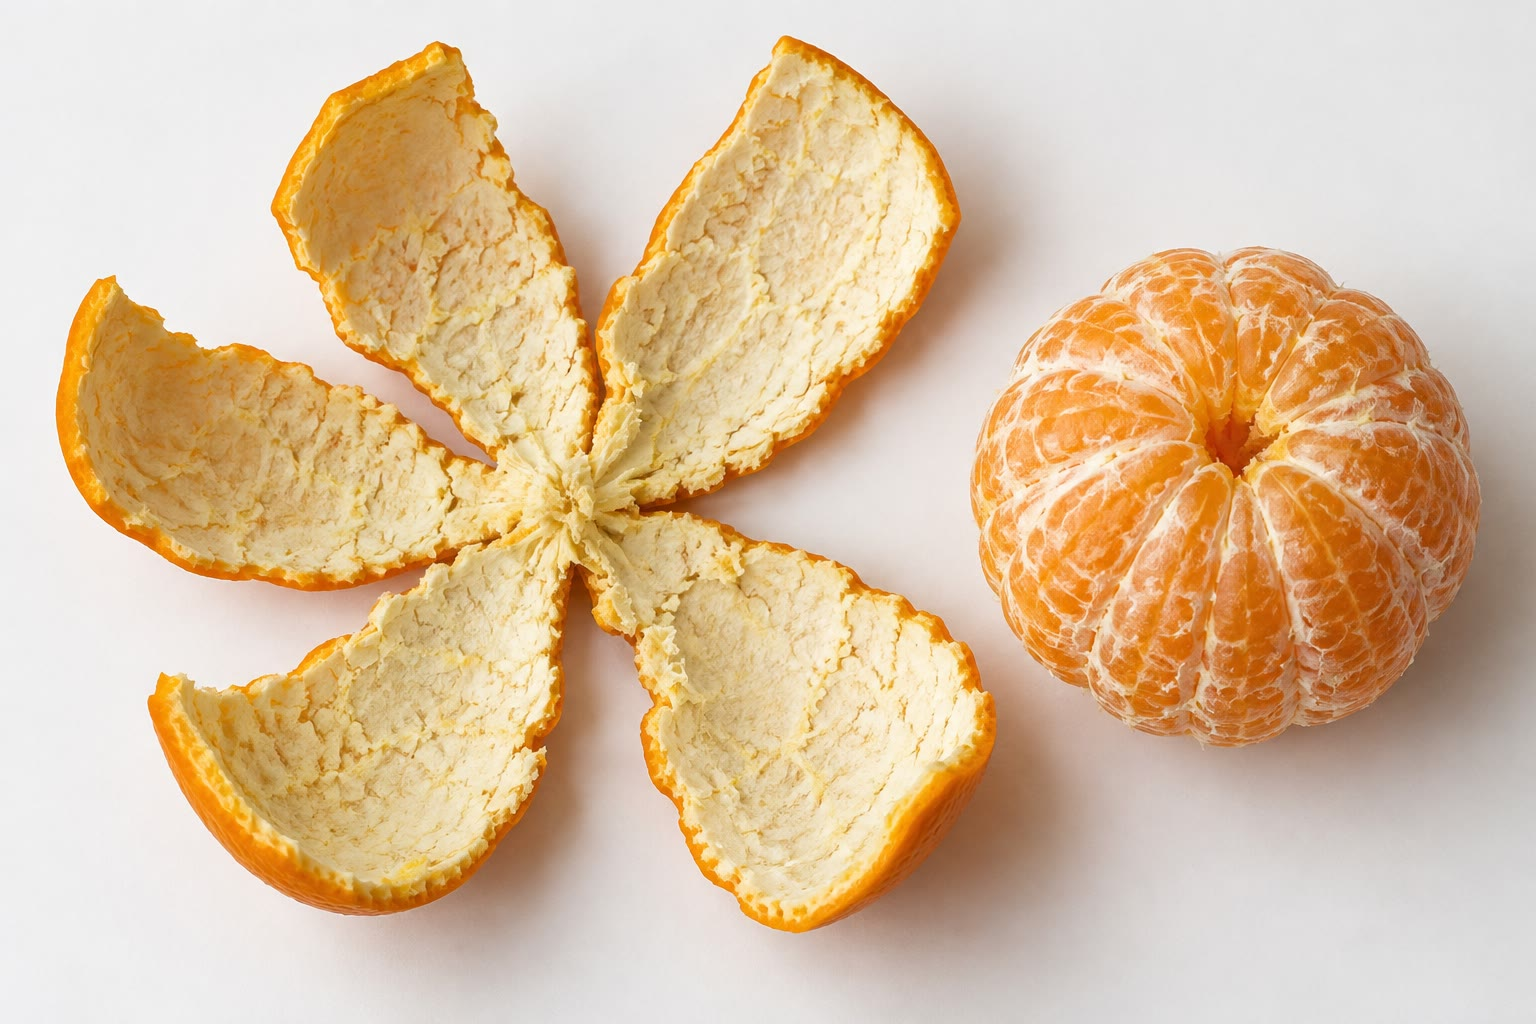
\includegraphics[width=0.4\linewidth]{images/book1/ai/g3-orange-peel.jpg}

{\small Kulit jeruk tidak bisa terletak datar tanpa robek.}
\end{omfigure}

\begin{remark}[Peta dan bola dunia tidak sepakat]\label{rem:g3:continents-and-oceans:disagree}
Pada \omterm{def:g3:continents-and-oceans:world-map}{peta dunia} ini, Antarktika tampak seperti salah satu \omterm{def:g3:continents-and-oceans:continent}{benua} terbesar,
terentang di sepanjang tepi bawah. Pada \omterm{def:g3:continents-and-oceans:globe}{bola dunia}, Antarktika adalah
daratan yang bundar, lebih kecil daripada Amerika Selatan. Di dekat \omterm{def:g3:continents-and-oceans:poles}{kutub},
\omterm{def:g2:drawing-to-map:map}{peta} datar sangat meregangkan daratan. Di dekat \omterm{def:g3:continents-and-oceans:equator}{khatulistiwa}, peregangannya
sangat sedikit. Jika kamu ingin membandingkan ukuran dua tempat yang jauh
dari \omterm{def:g3:continents-and-oceans:equator}{khatulistiwa}, bola dunialah yang menunjukkan kebenaran.
\end{remark}

\begin{method}[Membaca peta dunia]\label{met:g3:continents-and-oceans:reading}
Pada \omterm{def:g3:continents-and-oceans:world-map}{peta dunia} seperti ini:
\begin{enumerate}
  \item utara ada di atas, selatan di bawah; \omterm{def:g3:continents-and-oceans:poles}{Kutub Utara} adalah seluruh tepi
        atas dan \omterm{def:g3:continents-and-oceans:poles}{Kutub Selatan} seluruh tepi bawah;
  \item \omterm{def:g3:continents-and-oceans:equator}{khatulistiwa} adalah garis yang melintang di tengah: semua yang ada
        di atasnya berada di \omterm{def:g3:continents-and-oceans:equator}{belahan bumi utara}, semua yang ada di bawahnya
        di \omterm{def:g3:continents-and-oceans:equator}{belahan bumi selatan};
  \item tepi kiri dan tepi kanan adalah garis yang sama pada \omterm{def:g3:continents-and-oceans:globe}{bola dunia}:
        kapal yang berlayar keluar dari tepi kanan muncul kembali di kiri.
\end{enumerate}
\end{method}

\section{Latihan}

\begin{exercise}[$\star$]\label{exo:g3:continents-and-oceans:1}
Sebutkan ketujuh \omterm{def:g3:continents-and-oceans:continent}{benua}. Mana yang terbesar? Mana yang terkecil?
\end{exercise}

\begin{exercise}[$\star$]\label{exo:g3:continents-and-oceans:2}
Sebutkan kelima \omterm{def:g2:water-on-earth:ocean}{samudra}. Mana yang terbesar? Mana yang terkecil?
\end{exercise}

\begin{exercise}[$\star$]\label{exo:g3:continents-and-oceans:3}
Salin dan isilah dengan ``\omterm{def:g3:continents-and-oceans:poles}{Kutub Utara}'', ``\omterm{def:g3:continents-and-oceans:poles}{Kutub Selatan}'', atau
``\omterm{def:g3:continents-and-oceans:equator}{khatulistiwa}'': \dots{} ada di bagian atas \omterm{def:g3:continents-and-oceans:globe}{bola dunia}; \dots{} ada di
bagian bawah; \dots{} melingkari bagian tengahnya.
\end{exercise}

\begin{exercise}[$\star$]\label{exo:g3:continents-and-oceans:4}
\omterm{def:g3:continents-and-oceans:equator}{Belahan bumi utara} atau selatan? Eropa; Australia; Antarktika; Amerika
Utara.
\end{exercise}

\begin{exercise}[$\star$]\label{exo:g3:continents-and-oceans:5}
\omterm{def:g2:water-on-earth:ocean}{Samudra} mana yang terletak di sekitar \omterm{def:g3:continents-and-oceans:poles}{Kutub Utara}? \omterm{def:g2:water-on-earth:ocean}{Samudra} mana yang
terletak di sekitar Antarktika?
\end{exercise}

\begin{exercise}[$\star\star$]\label{exo:g3:continents-and-oceans:6}
\omterm{def:g2:water-on-earth:ocean}{Samudra} mana yang kamu lintasi untuk pergi dari Afrika ke Amerika Selatan?
Dari Australia ke Amerika Selatan, ke arah timur? Dari Afrika ke Australia?
\end{exercise}

\begin{exercise}[$\star\star$]\label{exo:g3:continents-and-oceans:7}
Sam tinggal di sebuah negara yang panas sepanjang tahun. Bo tinggal di
sebuah stasiun penelitian yang membeku sepanjang tahun. Salah satu dari
mereka tinggal di dekat \omterm{def:g3:continents-and-oceans:equator}{khatulistiwa}, yang lain di dekat \omterm{def:g3:continents-and-oceans:poles}{kutub}. Siapa
tinggal di mana?
\end{exercise}

\begin{exercise}[$\star\star$]\label{exo:g3:continents-and-oceans:8}
Lena memutar \omterm{def:g3:continents-and-oceans:globe}{bola dunia} 10 kali. Jarinya mendarat di \omterm{def:g2:water-on-earth:ocean}{laut} 7 kali. Berapa
kali jarinya mendarat di daratan? Apakah ini sesuai dengan dugaanmu?
Mengapa?
\end{exercise}

\begin{exercise}[$\star\star$]\label{exo:g3:continents-and-oceans:9}
Pada \omterm{def:g3:continents-and-oceans:world-map}{peta dunia} di halaman~\pageref{fig:g3:continents-and-oceans:world-map},
\omterm{def:g2:water-on-earth:ocean}{Samudra} Pasifik muncul dua kali. Mengapa? Apakah Bumi yang sebenarnya
mempunyai dua \omterm{def:g2:water-on-earth:ocean}{Samudra} Pasifik?
\end{exercise}

\begin{exercise}[$\star\star\star$]\label{exo:g3:continents-and-oceans:10}
Tom berkata: ``Pada \omterm{def:g3:continents-and-oceans:world-map}{peta dunia}, Antarktika lebih panjang daripada Asia,
jadi Antarktika adalah \omterm{def:g3:continents-and-oceans:continent}{benua} terbesar.'' Apakah Tom benar? Pakailah daftar
\omterm{def:g3:continents-and-oceans:continent}{benua} dari yang terbesar sampai yang terkecil, dan jelaskan mengapa \omterm{def:g3:continents-and-oceans:world-map}{peta
dunia} itu mengecohnya.
\end{exercise}
